% kapitel2.tex
\chapter{Grundlagen}
\label{chapter:kap2}

\section{Simulationsstudien}

\begin{figure}[h]
	\centering
	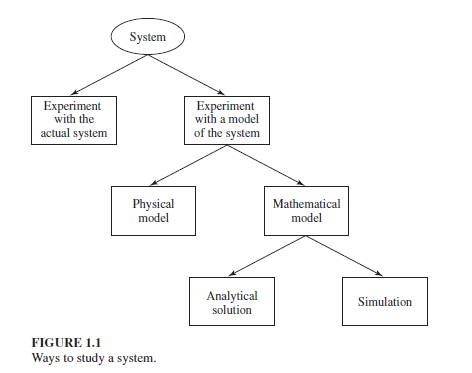
\includegraphics[width=8cm]{bilder/system_study}
	\caption{Arten von Systemstudien}
  \label{fig:sysstudy}
\end{figure}

\subsection{M/M/1-Modell}

\begin{figure}[h]
	\centering
	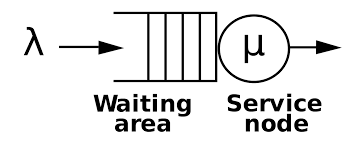
\includegraphics[width=8cm]{bilder/mm1}
	\caption{M/M/1 Warteschlangenmodell}
  \label{fig:mm1}
\end{figure}

% Verteilung der Zeitabstände zwischen Kunden
\begin{equation}
f_T(x) = \lambda e^{- \lambda t}, \quad t \geq 0
\end{equation}

% Verteilung der Zeitabstände zwischen Services
\begin{equation}
f_S(x) = \mu e^{- \mu t}, \quad t \geq 0
\end{equation}

\begin{figure}[h]
	\centering
	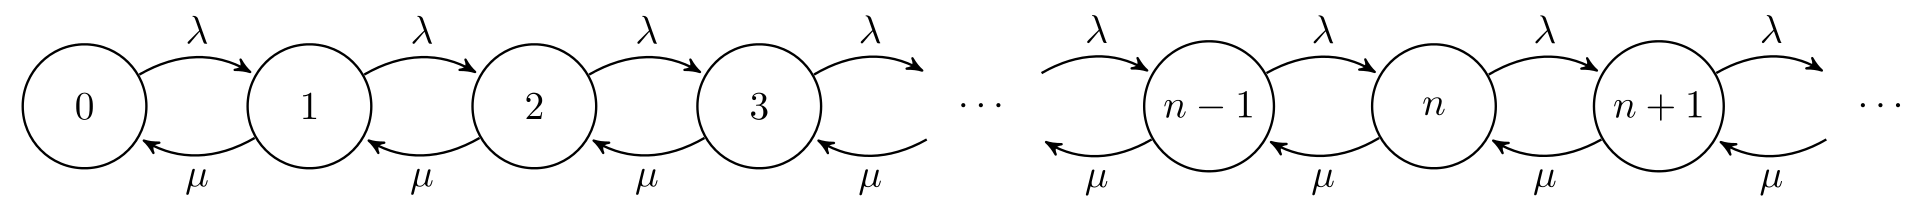
\includegraphics[width=8cm]{bilder/mm1_state}
	\caption{M/M/1 Zustandsübergangsdiagramm}
  \label{fig:mm1_state}
\end{figure}

% Verteilung für die Anzahl von Kunden im System
\begin{equation}
P_n = (1 - \rho) \rho^n
\end{equation}

% Erwartete Anzahl von Kunden im System
\begin{equation}
L = \frac{
	\rho
}{
	1 - \rho
} = \frac{
	\lambda
}{
	\mu - \lambda
}
\end{equation}

% Erwartete Wartezeit in der Queue
\begin{equation}
W_q = \frac{
	\rho
}{
	\mu - \lambda
} = \frac{
	\lambda
}{
	\mu ( \mu - \lambda )
}
\end{equation}

\section{Parameter-Schätzer}

% Regressionsfunktion
\begin{equation}
y_i = \eta(x_i, \theta)+ \epsilon_i, \quad i=1,2,...,n
\end{equation}

% Verteilung der Residuen
\begin{equation}
\epsilon \sim N(0, \sigma^2)
\end{equation}

% Erwartungswert der Daten soll die Regression sein
\begin{equation}
E(y | x) = \eta(x, \theta)
\end{equation}

% Schätzer
\begin{equation}
\hat{y} = \eta(x, \hat{\theta})
\end{equation}

% Kleinsten Quadrate
\begin{equation}
\underset{\theta \in \mathcal{R}}{\arg\min} \sum_{i=1}^n \left[ \eta(x_i,\theta) - y_i \right]^2
\end{equation}

% M estimator
\begin{equation}
\sum_{i=1}^n \psi(y_i, \theta) = 0
\end{equation}

\subsection{Maximum-Likelihood-Schätzer}

% Likelihood
\begin{equation}
\mathit{Lik}(\theta, y) = \prod_{i=1}^n f(y_i, \theta)
\end{equation}

% log Likelihood
\begin{equation}
L(\theta, y) = \log \prod_{i=1}^n f(y_i, \theta) = \sum_{i=1}^n \log f(y_i, \theta)
\end{equation}

\begin{equation}
\frac{\partial}{\partial \theta} L(\theta, y) = \sum_{i=1}^n \frac{\partial}{\partial \theta} \log f(y_i, \theta) = 0
\end{equation}

\begin{equation}
\psi = \frac{ -f }{ f }
\end{equation}

\begin{equation}
\mathrm{Var}(\theta) = \left[ I(\theta) \right]^{-1}
\end{equation}

\begin{equation}
I(\theta) = E \left(- \frac{\partial^2}{\partial \theta^2} L(\theta, y) \right) 
\end{equation}

\begin{equation}
\mathrm{Var}(\hat{\theta}) \approx \left[ \left. - \frac{\partial^2}{\partial \theta^2} L(\theta, y) \right|_{\theta = \hat{\theta}} \right]^{-1}
\end{equation}

\section{GoF-Tests}

\subsection{Kolmogorov-Smirnov Test}

\begin{equation}
D = \underset{y_i}{\sup} \{ F_n(y_i) - F(y_i, \theta) \}
\end{equation}

\subsection{Anderson-Darling Test}

\begin{equation}
A^2 = -n - \sum_{i=1}^n \frac{2 i - 1}{n} \left[ \log F(y_i, \hat{\theta}) + \log( 1 - F(y_{n+1-i}, \hat{\theta})) \right]
\end{equation}

\subsection{Chi-Quadrat Test}

\section{Konfidenzintervalle}

% Erwartete Wartezeit in der Queue für allgemeinere M/G/1 Systeme
\begin{equation}
W_q = \frac{
	\lambda \left[ \mathrm{Var}(S) + (E(S))^2 \right]
}{
	2 (1 - \lambda E(S)) 
}
\end{equation}

\section{Konfidenzbänder}

\section{Coverage Error}

\section{Resampling Verfahren}

\subsection{Bootstrap}























